\chapter{Learning Programming}
\label{chap:learning-programming}

% TODO: Rephrase (avoid "this chapter describes")
This chapter describes the current state of the art of teaching programming, both from the view of successful learning systems and from the view of the research on learning programming.

\section{Existing Systems for Learning Programming}
\label{sec:existing-systems}

% TODO: Rephrase (avoid "presented"?)
There are many systems for learning programming and they differ from each other
in several significant aspects, which are presented in \cref{tbl:existing-systems-categorization}.

\begin{table}[htb]
\centering
\begin{tabular}{l l}
\toprule
Aspect & Examples \\
\midrule
Tangibility & computer applications, physical toys \\
%Target group & primary school, high school students \\
  % Target group interacts with prerequisites
Prerequisites & reading, typing, mathematics \\
Content & loops, variables, functions \\
Form & tasks, videos, texts \\ % worked-out examples,
Tasks & robot on grid, drawing with turtle \\
% Playing-learning ratio & mostly playing, mostly learning \\
Programming language & block-based, textual \\
Adaptivity & task recommendation, mastery learning \\
%Price & free, paid
\bottomrule
\end{tabular}
\caption{Differentiating aspects of systems for learning programming.}
\label{tbl:existing-systems-categorization}
\end{table}


% TODO: Consider to add an interesting fact/observation after the table,
% (or possibly citation pointing to some more broad overviews);
% (linking the table to the rest of the section)
% and consider to move the following "meta-information" to the chapter intro.
The rest of this section briefly describes the most notable existing systems,
focusing on their features that improve learning or engagement.
Section \ref{sec:strategies-for-easier-learning} then extrapolates useful
strategies for teaching programming.


\subsection{LightBot}
\label{sec:lightbot}
LightBot%
\footnote{Available at \url{http://lightbot.com/}.}
is a mobile and web application offering a fixed sequence of tasks solved by
a block-based programming language
(\cref{fig:lightbot}).
%(figure \ref{fig:lightbot-instruction}).
Students create short programs to control a robot in a grid world.
The robot can not only walk and turn left or right, but also jump and turn on lights.
Having five different basic actions is useful for diversity of elementary tasks.
The system covers sequences of commands, procedures, simple loops via tail-recursion,
and conditional commands.

%\subsection{Robozzle}
%\label{sec:robozzle}
%With a robot on a grid and block-based programming, Robozzle%
%  \footnote{Available at \url{http://www.robozzle.com/}.}
%  is similar to LightBot;
%however, it adds a new feature: colored fields.
%Colors can be used in conditional commands,
%  which allows for hundreds of diverse tasks,
%  including difficult tasks with sophisticated recursion.
%Robozzle also allows users to create their own tasks,
%  which can be tried and rated by other learners.
%
%\imgW[0.8]{robozzle}{Robozzle.}


\subsection{Problem Solving Tutor}
\label{sec:problem-solving-tutor}
Problem Solving Tutor%
\footnote{Available at \url{tutor.fi.muni.cz}.}
includes a few problem sets for practicing programming,
such as Interactive Python, Karel the Robot, or Robotanist
% TODO: more precise description of the tasks instead of e.g. "Inter. Python",
% see the reffed paper for inspiration.
\cite{proso}.
Robotanist (\cref{fig:robotanist}) is similar to LightBot,
with an addition of colored fields.
Colors can be used in conditional commands, which allows for diverse tasks,
including difficult problems with complex recursion.  After
each solved task, Problem Solving Tutor shows a recommendation for two next
tasks %(one easier, on more difficult),
with predicted solving times.
Showing predicted time % to the user
serves as a motivational element, posing
a suitable challenge to overcome oneself
\cite{pelanek-student-modeling-times}.

%\imgW[0.6]{lightbot}{LightBot.}
%\imgW{lightbot-instruction}{LightBot provides clear and simple interactive instructions.}
%\imgW[0.6]{robotanist}{Robotanist in Problem Solving Tutor, Detour task.}


\begin{figure}[htb]
\centering
\begin{subfigure}[t]{0.5\textwidth}
\centering
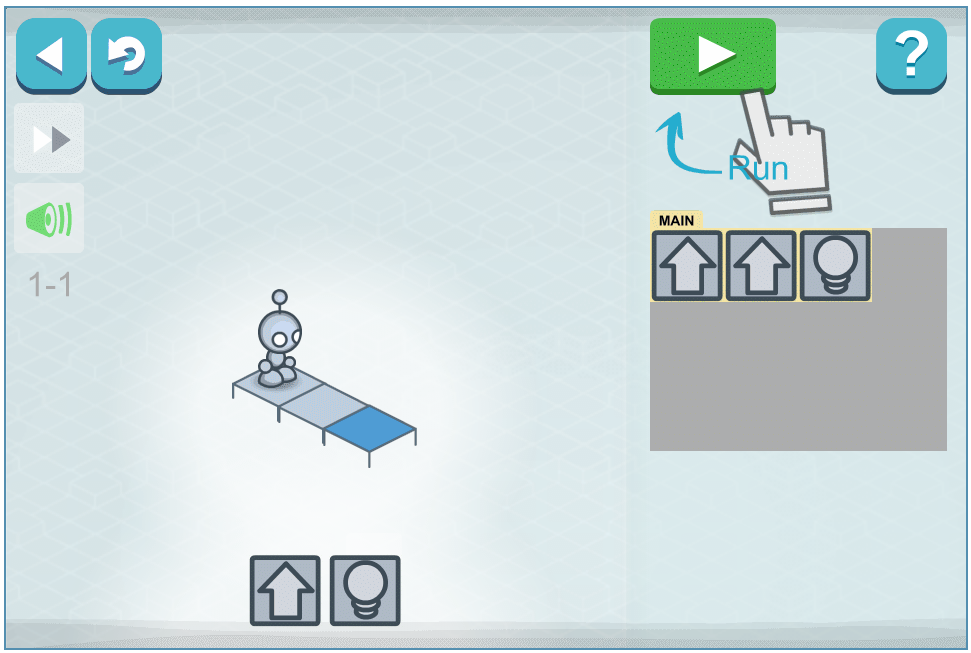
\includegraphics[height=4cm]{img/lightbot-instruction}
\caption{LightBot}
\label{fig:lightbot}
\end{subfigure}%
\begin{subfigure}[t]{0.5\textwidth}
\centering
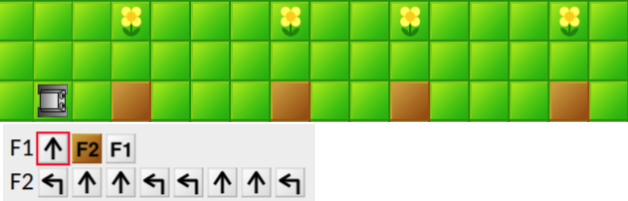
\includegraphics[height=4cm]{img/robotanist}
\caption{Robotanist}
\label{fig:robotanist}
\end{subfigure}
\caption{LightBot and Robotanist provide square grids for commands.}
\label{fig:lightbot-robotanist}
\end{figure}



\subsection{Blockly Games}
\label{sec:blockly-games}
Blockly is a popular block-based programming interface.
In contrast to the blocks in LightBot,
Blockly blocks can be assembled in nested control structures
(\cref{fig:blockly-games}).
Blockly Games%
\footnote{Available at \url{https://blockly-games.appspot.com/}.}
% TODO: Replace by figure using nested control structures
% and move the fre to the end of previous sentence.
%(figure \ref{fig:blockly-instruction})
%demonstrate Blockly usage. The webpage ...
consist of several problem sets with Blockly, ordered by increasing difficulty.
For example, in the first level, students learn how to compose blocks together
as a puzzle, and in the second level they learn loops and conditions by solving
tasks in a maze. Final level serves as a transition from block-based
programming to textual programming in JavaScript.
Each level consists of 5-10 tasks, again ordered by increasing difficulty. %, with no personalization.
The fixed order enables to build on the program from the previous task,
thus gradually leading to more complex programs,
resulting for example in sophisticated images in turtle graphics.
Blockly Games includes non-ignorable interactive instructions,
which require to take a described action before they disappear
\cite{blockly-10-things}.

%\imgW[0.7]{blockly-instruction}%
%  {Blockly Games includes non-ignorable interactive instructions, %
%  which require to take a described action before they disappear.}

\subsection{Hour of Code}
\label{sec:hoc}
Hour of Code%
\footnote{Available at \url{https://hourofcode.com}.}
%(figure \ref{fig:hour-of-code-sw})
provides many one-hour tutorials, each containing about 15 tasks in fixed order,
using Blockly-based language
(\cref{fig:hoc}).
These tutorials focus on motivation, using themes from popular movies and
games, and providing videos with famous people explaining programming concepts.
The tutorials use high-level theme-specific blocks, such as ``set droid to a
random speed``, and they are restricted to only one or two programming
concepts, e.g. sequences of commands and events.
In some tasks, the built program is not a direct solution for a robot,
but rather a game, in which the code specifies actions triggered on events.
% TODO: There is some space to include more info about HoC.

%\imgW[0.7]{hour-of-code-sw}{Hour of Code, Star Wars tutorial.}


\begin{figure}[htb]
\centering
\begin{subfigure}[t]{0.43\textwidth}
\centering
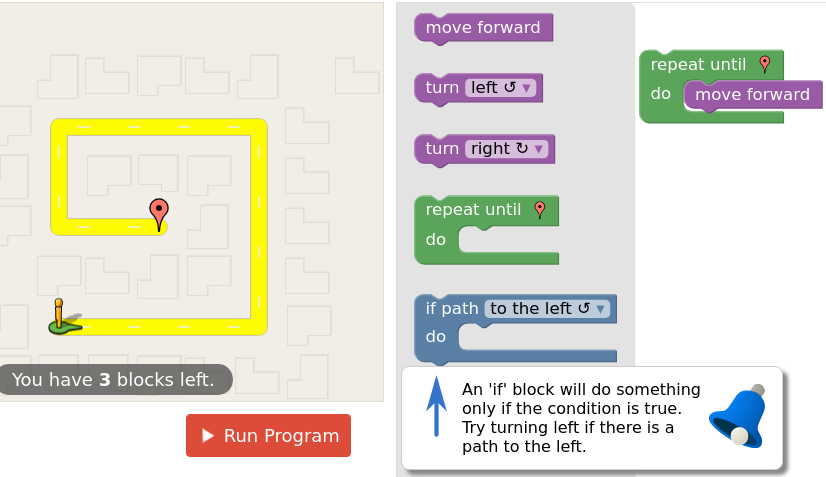
\includegraphics[height=33mm]{img/blockly-nested}
\caption{Blockly Games (Maze level)}
\label{fig:blockly-games}
\end{subfigure}%
~
\begin{subfigure}[t]{0.57\textwidth}
\centering
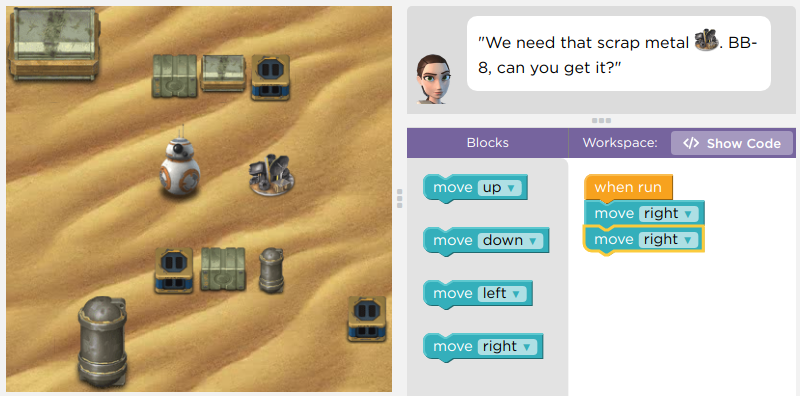
\includegraphics[height=33mm]{img/hour-of-code-sw}
\caption{Hour of Code (Star Wars theme)}
\label{fig:hoc}
\end{subfigure}
\caption{Two programming games using nested blocks.}
\label{fig:blockly-hoc}
\end{figure}





\subsection{Human Resource Machine}
\label{sec:human-resource-machine}
Human Resource Machine%
\footnote{\url{http://tomorrowcorporation.com/human-resource-machine-hour-of-code-edition}}
%\footnote{Free Hour of Code edition available at \url{http://tomorrowcorporation.com/human-resource-machine-hour-of-code-edition}.}
is an example of an offline computer game for learning programming.
%Although it is presented as a game,
%the player spends nearly all the time solving tasks similar to those in the previously mentioned learning systems.
% Removal candidate (1 sentence):
The sequence of tasks is non-personalized and nearly linear,
with a few short side branches.
Similarly to the systems above, it also uses block-based programming,
but now in a different domain:
it offers low-level programming commands, such as
input, output, move-from, move-to, add, or jump
%(figure \ref{fig:human-resource-machine}).
(\cref{fig:hrm}).
% input, output, move-to, move-from, add, sub, jump, jump-nonzero, jump-negative.
The programming environment includes a debugger,
providing a possibility to step through the program.
All concepts are explained when they first appear in the game,
and programming blocks can
be explained again simply by dragging the block onto a dedicated field with a question
mark.

%\imgWithFootnote[0.7]{human-resource-machine}{Human Resource Machine}%
%{Source: \url{https://tomorrowcorporation.com/humanresourcemachine}}
%%{Source: \url{https://tomorrowcorporation.com/humanresourcemachine} (Tommorow Corporation).}

\subsection{Khan Academy}
\label{sec:khan-academy}
Khan Academy has a computer programming curriculum%
\footnote{Available at \url{https://www.khanacademy.org/computing/computer-programming}.}
that uses textual programming in JavaScript with functions for drawing shapes
in absolute coordinates %(figure \ref{fig:khan-academy}).
(\cref{fig:ka}).
In addition to programming tasks, it contains text and video explanations, and
projects. Some videos are in the form of interactive \emph{talk-throughs},
in which the student can fiddle with the explained code at any moment to understand
how it works.

%\imgW[0.8]{khan-academy}%
%  {Parting Clouds programming task on Khan Academy.}


\begin{figure}[htb]
\centering
\begin{subfigure}[t]{0.48\textwidth}
\centering
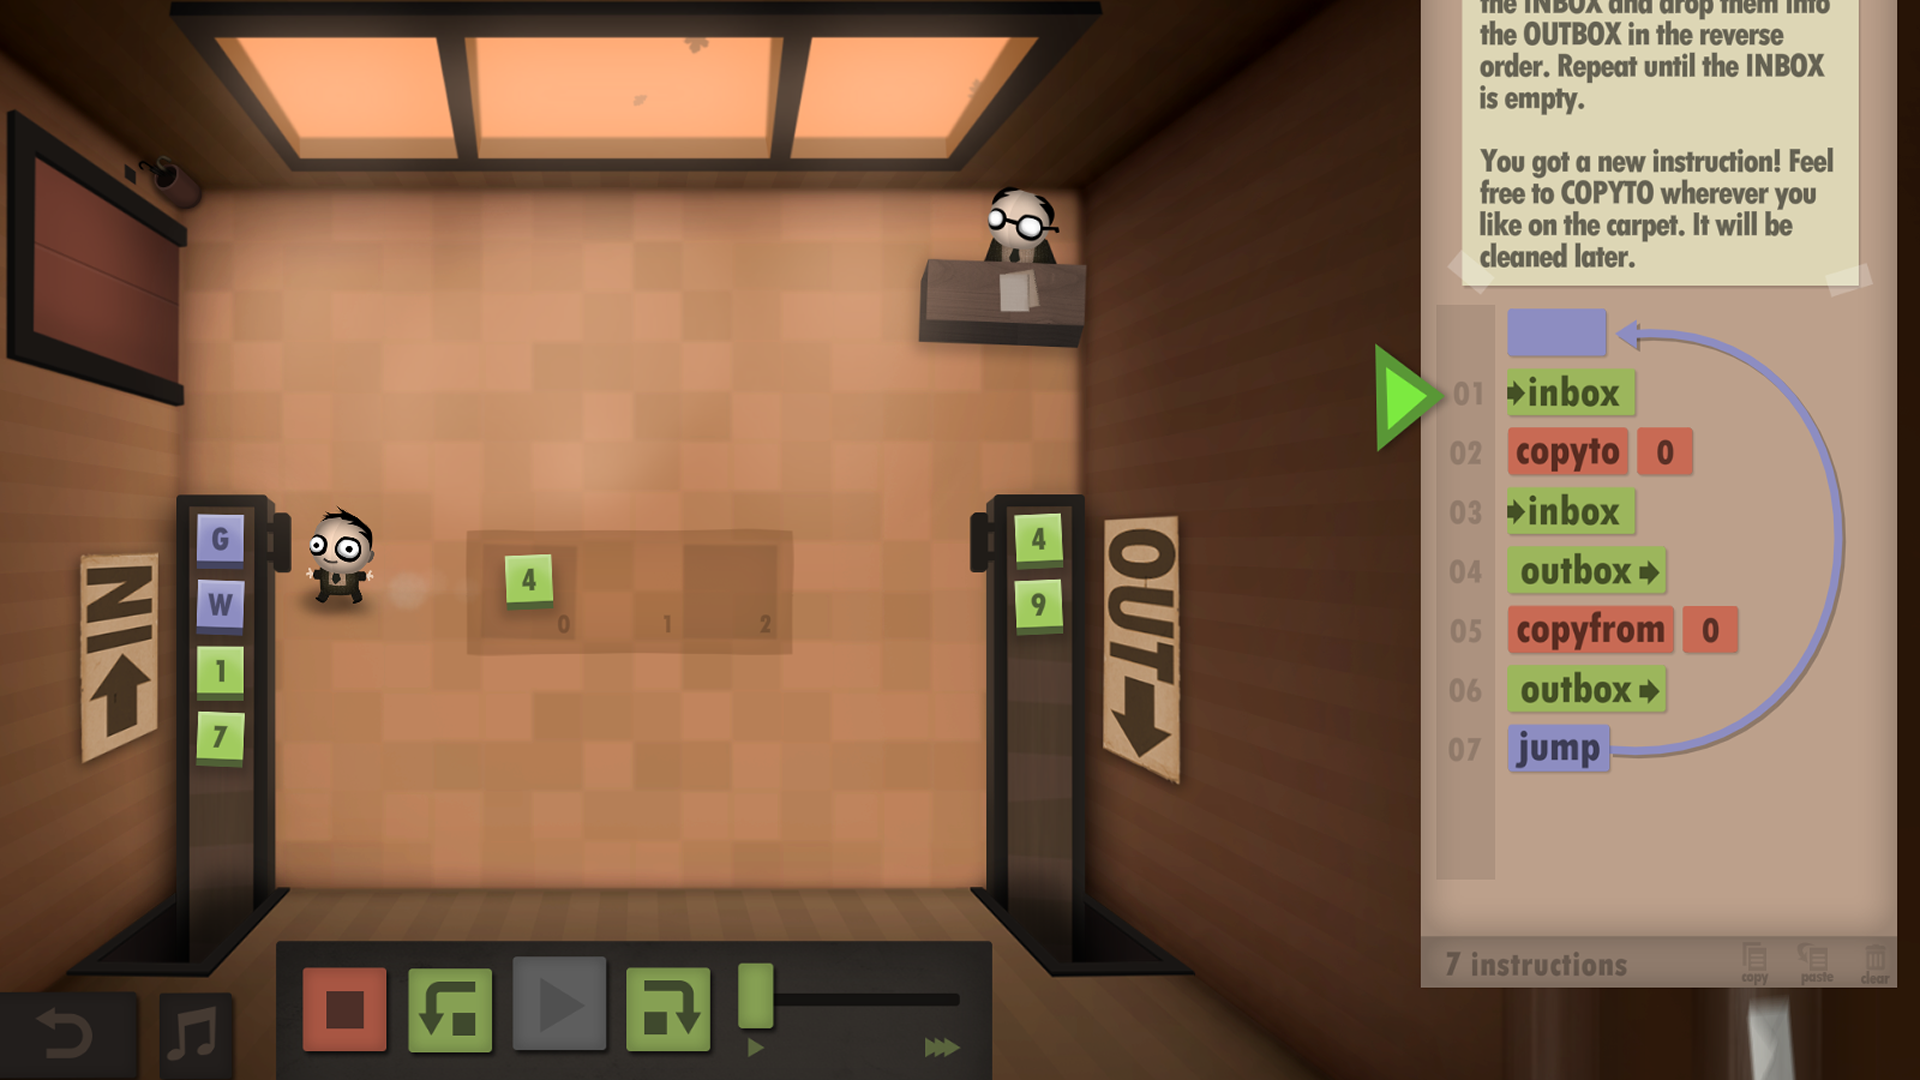
\includegraphics[height=30mm]{img/human-resource-machine}
\caption{Human Resource Machine\protect\footnotemark}
\label{fig:hrm}
\end{subfigure}%
\begin{subfigure}[t]{0.52\textwidth}
\centering
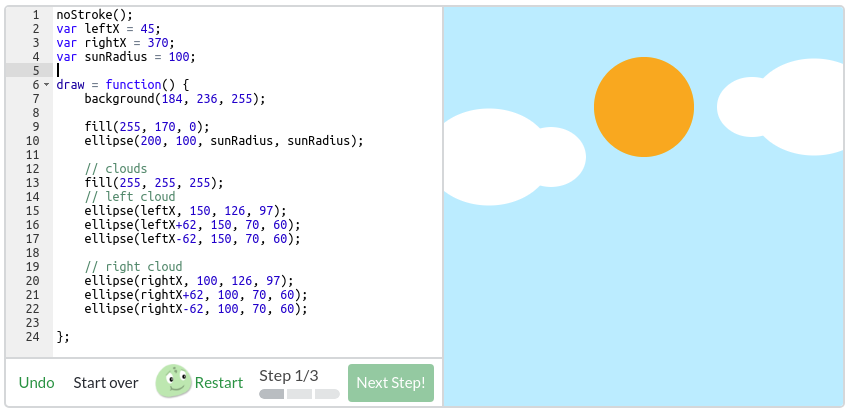
\includegraphics[height=30mm]{img/khan-academy}
\caption{Khan Academy}
\label{fig:ka}
\end{subfigure}
\caption{Tasks using Assembly-based and JavaScript-based languages.}
\label{fig:hrm-ka}
\end{figure}
\footnotetext{Source: \url{https://tomorrowcorporation.com/humanresourcemachine}.}






%\subsection{We Can Code}
%\label{sec:umime}
%
%TODO: present UmimeProgramovat -> turtle graphics, mastery learning
%\footnote{Available at \url{https://www.umimeprogramovat.cz/} (Czech only).}


%\subsection{Ozobot}
%\label{sec:ozobot}
%Ozobot%
%\footnote{Product webpage available at \url{http://ozobot.com/}.}
%is a small physical robot
%programmable by either a Blockly-based interface,
%  or even without a computer
%  by drawing lines on a paper and reading them with a color sensor on the robot.
%As it does not require ability to read and write
%  Ozobot is suitable for even very young children.

%\imgWithFootnote[0.8]{ozobot-robot}{Ozobot}%
%{Source: \url{https://www.flickr.com/photos/robpegoraro/19464353039}, Rob Pegoraro.}

%\imgW{ozobot}{%
%  Ozobot simulator (available at \url{http://games.ozoblockly.com}) %
%  is a Blockly-like interface for creating programs for Ozobot %
%  (but the simulater requires the ability to read). %
%  It also includes a few prepared tasks.}


%\subsection{Project Euler}
%\label{sec:project-euler}
%The core of Project Euler%
%\footnote{Available at \url{projecteuler.net}.}
%is a list of several hundreds of programming problems with one correct answer.
%The problems can be solved in any language
%and then checked whether the computed answer is correct.
%The project is not meant to teach elementary programming,
%but rather to hone one’s programming skills;
%more complicated tasks even require some knowledge of algorithms and data structures.
%
%\imgW[0.7]{project-euler-progress}{%
%Project Euler provides several means of motivation: %
%levels (based purely on number of solved tasks), badges %
%(e.g. for solving 10 consecutive problems, 50 prime numbered problems, etc.), %
%comparison with user’s friends, %
%statistics page with several leaderboard (e.g. by country), %
%and a special score based on the performance on the most recently published problems.}


%\subsection{HackerRank}
%\label{sec:hacker-rank}
%
%Online programming contests,
%in which people attempt to solve as many problems as possible
%in limited time frame of a few hours,
%became popular in the last years.
%In addition to organizing such contests regularly,
%HackerRank%
%\footnote{Available at \url{https://www.hackerrank.com/}.}
%also provides many training programming tasks for various topics,
%from introductory programming to machine learning.
%% Solutions are evaluated on a server against a prepared set of test cases with time limits.
%In addition to the classic motivation in the form of points, badges and leaderboards, students are motivated to practice to perform well in the competitions,
%where they can win some prizes and sometimes even job offers.
%HackerRank also helps student to decide on a problem to solve by showing its difficulty according to the author of the task (on a 3-star scale),
%as well as success rate among the past submissions.
%Furthermore, after solving a task,
%a specific recommendation the next task to solve is shown.


%\imgW[0.6]{hackerrank}{HackerRank. %
%Each task specifies input and output format, including some examples. %
%Solution can be written either locally or in the provided online editor.}


\section{Strategies to Support Learning}
%\section{Strategies for Easier Learning}
\label{sec:strategies-for-easier-learning}

Learning programming is difficult,
  because it requires
  to adopt algorithmic thinking,
  understand program execution,
  and remember formal syntax of a programming language;
  all these three skills at once. % at the same time.
To make learning easier,
  the systems presented in the previous section use diverse strategies,
  such as avoiding syntax errors,
  displaying visual output
  and providing hints.
Various other strategies were tried in the past as well;
article \emph{Lowering barriers for Novice Programmers}
  \cite{lowering-barriers}
  provides a detailed overview.


\subsection{Avoiding Syntax Errors}
\label{sec:avoiding-syntax-errors}

A common strategy for avoiding syntax errors is to replace textual programming
with drag-and-drop block-based programming.
There are two basic types of block-based interfaces:
  either with a square grid defining the program shape,
  often one row per function
  (\cref{fig:lightbot-robotanist}),
  or the blocks can be nested and assembled arbitrarily,
  with no limit on maximum program length,
  often one vertical stack per function
  (\cref{fig:blockly-hoc}).
The fixed square grid is simpler to understand and manipulate with,
  but it does not allow for nesting,
  which is a fundamental feature of computer programs.
This restriction is usually overcome by
  combining condition and commands into a single block,
  by using recursion instead of loops,
  and by replacing nested sequences of commands by a new function.

%TODO: the block-based editors are a special case of "structred editors",
%idea: editor only allows edits that transform the code from one syntactically correct
%program to another (basically working on AST level, edit = transforms to another AST)
%(compared to: classical text editors, where the edit can be arbitraty, making the code
%not syntactically correct).

%\subsection{Potential Drawback of Block-based Interfaces}
%\label{sec:potential-drawback-of-block-based-interfaces}
A drawback of using block-based programming
  is that the students need to learn a proper textual programming language in
  the future to be able to implement more complex programs.
Several controlled experiments were performed to test a hypothesis
  that it is still beneficial to start an introductory programming course
  with a block-based programming,
  even when the students will be writing textual code later in the course
  \cite{comparing-blocks-text-price2015, comparing-blocks-text-weintrop2017}.
Results suggest that block-base interfaces indeed lead to increased learning and
motivation; however, the evidence is not fully convincing. For example, in
some of these studies, the programming interfaces differed in more aspects than
just in using blocks instead of text. Furthermore, these studies do not
answer when it is the right moment to switch from block-based to textual
programming.

%\subsection{Transition Strategy}
%\label{sec:transition-strategy}
%Weintrop and Wilensky suggest that the block representation of the code
To make the transition easier, block representation of the code
  should match the underlying programming language
  to which the student is expected to move in the next phase
  \cite{challenges-of-blocks-based-environments}.
However, resemblance to a programming language sometimes
  conflicts with the readability of the blocks for novices.
Instead of making compromises,
  the system can progressively change the available set of blocks in each level,
  making them more and more similar to a textual programming language.
In the last level of Blockly Games, which employ this strategy,
  the text on the blocks matches the generated JavaScript exactly
  \cite{blockly-10-things}.

%TODO:
%- note: "blending block-based and text-based programming approaches (e.g., Pencil Code
%(Bau 2015), Tiled Grace (Homer and Noble 2014), and Greenfoot’s Frame-based editor (Kölling et al.
%2015)"


\subsection{Visual Output}
\label{sec:visual-output}

Learning systems can help students to track program execution
  by providing a clear visual representation of the current state
  and effects performed by the program.
This can be achieved naturally for turtle graphics,
  where the whole state is just a position and orientation of the turtle,
  and effects are the drawn lines.
Similarly, in simple games, such as those described in
  \cref{sec:lightbot,sec:problem-solving-tutor,sec:blockly-games,sec:hoc},
  the grid world visualization contains complete information about the current
  state (\cref{fig:lightbot-robotanist,fig:blockly-hoc}).
For the simplicity of their visual output,
  drawings and grid world games have become prevalent task types
  in the current systems for learning programming.

\subsection{Instructions and Hints}
\label{sec:instructions-and-hints}

Most educational systems include instructions
  to explain new concepts such as loops and conditions.
%However, Neil Fraser explains that students ignore instructions,
However, many students ignore instructions,
  no matter how prominent they are \cite{blockly-10-things}.
A solution to this problem are actionable non-ignorable instructions,
  which cannot be closed manually by the student, and disappear only once the
  student performs the action described in the instruction
  (\cref{fig:blockly-games}).

In addition to the instructions, some systems offer hints, which appear either
  upon a student request, or automatically after a certain time of unsuccessful
  solving. Although it is possible to generate a hint in any state,
  using data of students which have successfully solved the task before
  \cite{generating-hints}, the existing systems use a few manually prepared
  hints, instead of relying on the automatic approaches.

\section{Strategies to Support Motivation}
%\section{Strategies for Motivation}
\label{sec:motivation}
% NOTE: Prev section: learning, this section: engagement.

In addition to strategies for easier learning presented in section
\ref{sec:strategies-for-easier-learning}, it is equally important to create an
engaging environment supporting students’ motivation.
All strategies for supporting motivation are based on fulfilling some human
needs \cite{nvc}. % TODO: cite specific page
\Cref{tbl:motivation-strategies} links needs to common strategies.
% TODO? related: flow, happiness, switch-elephant (prev. section: path)

\begin{table}[htb]
\centering
\begin{tabular}{ll}
\toprule
Needs & Strategies \\
\midrule
Purpose & Emphasizing usefulness of the programming skill. \\ %, confidence
Progress, learning & Skills visualization, points, levels. \\
Effectiveness & Recommending tasks of optimal difficulty. \\ % concentration/flow
Autonomy & Allowing to choose a topic or a task. \\
Recognition & Badges, leaderboards. \\  %Appreciation  % leaderboard vs. scoreboard?
Sharing & Possibility to share programs or achievements. \\
Cooperation & Pair programming. \\
Beauty, harmony & Appealing game world. \\ %, which is nice to look at and fun to play with \\
Fun & Entertaining tasks. \\
Creativity & Open-ended tasks, projects. \\  %, self-expression
% Community?
\bottomrule
\end{tabular}
\caption{Needs and strategies that help to fulfill these needs.}
\label{tbl:motivation-strategies}
\end{table}



\subsection{Appealing Game World}
\label{sec:motivation.game-world}
Ideally, game world should appeal to students --
even without tasks to solve,
  it should be an interesting toy to play with \cite{book-of-lenses}.
That is why all Hour of Code tutorials are based on movies and games
  popular among children, such as Angry Birds, Frozen, or Star Wars
  (\cref{fig:hoc}).
In such environments, it is possible to assign open-ended tasks,
  or even let the students create whatever they want,
  which works well especially for creative students seeking for self-expression.
For example, Khan Academy programming curriculum contains many several
open-ended drawing projects (\cref{fig:ka}).
%\cref{sec:robomission.game-world}

\subsection{Entertaining Tasks}
\label{sec:motivation.tasks}
For many students, giving them specific small problems works better
  than large, loosely defined, open-ended tasks.
By solving small problems quickly,
  they get a feeling of progress and learning.
Another advantage of closed tasks
  is a more straightforward implementation of gamification features and adaptive behavior.

Small closed tasks result in short programs,
  but their behavior should be still interesting. % for the students to be satisfied.
To achieve complex behavior,
  a system can either provide students with macro-commands (e.g. to draw a circle)
  or with a skeleton of complex code, with a few gaps to fill in by students.
However, it is important for the students to feel ownership over the code,
  which is especially a concern with the code skeleton.
Solution implemented in Blockly Games
  is to make a series of tasks in which the students
  build on their program from the previous task
  \cite{blockly-10-things}.

% TODO: some examples in the form of figures + descriptions
% TODO: other important aspects: variability


\subsection{Optimal Challenge}  % OR: "Optimal Difficulty"
\label{sec:motivation.challenge}
For a great learning experience,
  difficulty of the task must match the skill of the student.
If the task it too easy,
  the student is not challenged and gets bored.
If the task is too difficult,
  the student becomes frustrated and desperate.
On the other hand, if the task has appropriate difficulty,
  the student is likely to be challenged and focused
  (\cref{fig:flow}).
The complete immersion into the task the student is solving at the moment is called
  a state of flow \cite{flow}
  or a \emph{zone of proximal development} \cite{zone-of-proximal-development}.
Achieving the state of flow maximizes the learning outcome \cite{adaptive-practice},
  and even increases the long-term level of happiness. % TODO: find a source of this claim
\Cref{chap:adaptive-learning} describes techniques for estimating student’s skill
  and show how to use that estimate for task recommendation and mastery learning.


\subsection{Gamification and Progress Visualization}

Sense of progress and learning can be boosted by visualizations of
progress towards mastery in the current topic, solved tasks, completed problems sets,
or acquired skills.
\Cref{fig:progress-visualization} shows examples of progress bars from various systems.

% TODO: cite relevant research, open learner model
% NOTE: also helps to decide what to practice next, while preserving student's
% autonomy (soft recommendation)

\begin{figure}[htb]
\centering
\begin{subfigure}{.48 \textwidth}
  \centering
  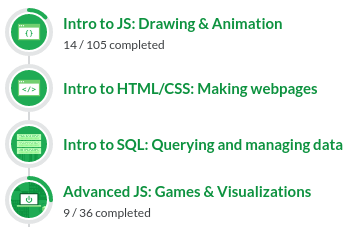
\includegraphics[width=.9\textwidth]{img/ka-skills}
\end{subfigure}
\begin{subfigure}{.48\textwidth}
  \centering
  
\includegraphics[width=.9\textwidth]{img/hour-of-code-progress}
  \bigskip
  \vspace{1mm}
  
\includegraphics[width=.9\textwidth]{img/umime-progressbar}
\end{subfigure}
\caption{%
  Progress bars: Khan Academy topics, Hour of Code tutorial,
  and mastery progress bar in Umíme Programovat (``We Can Code'').}
\label{fig:progress-visualization}
\end{figure}


%\subsection{Gamification}

Although the programming tasks themselves can be considered as a game
(e.g. Human Resource Machine from \cref{sec:human-resource-machine} is
presented purely as a game),
most learning systems add further gamification elements to increase the sense
of progress.
Common gamification elements include points, levels, badges, and leaderboards.

% TODO: figures: Project Euler, KA
% TODO: ref relevant research
